% +------------------------------------------------------------------------+
% | Reference manual page: Combinatorial_map_operations.tex
% +------------------------------------------------------------------------+
% | 04.02.2010   Guillaume Damiand
% | Package: Combinatorial_map
% +------------------------------------------------------------------------+
\ccRefPageBegin
%%RefPage: end of header, begin of main body
% +------------------------------------------------------------------------+

%--------------------------------------------------------------------------------
% \ccFunction{template < class CMap >
%   void remove_vertex_2(CMap& cm, typename CMap::Dart_handle dh);}
% {
%   Remove a 2D vertex, and merge eventually both incident edges.\\
% \ccCommentHeading{Parameters} \\
% \ccc{cm}: the combinatorial map used;\\
% \ccc{dh}: a dart belonging to the vertex to remove. 
% }
%--------------------------------------------------------------------------------
\begin{ccRefFunction}{is_removable<CMap,i>}
\ccInclude{CGAL/Combinatorial_map_operations.h}\\
\ccFunction{template <class CMap, unsigned int i>
    bool is_removable(const CMap& cm, typename CMap::Dart_const_handle dh);}
         {Returns true iff the \emph{i}-cell containing \ccc{dh} can be removed,
          i.e. if \ccc{i}==\ccc{CMap::dimension} or if 
          \ccc{i}==\ccc{CMap::dimension}-1 or 
          if \ccc{i}\mylt{}\ccc{CMap::dimension}-1 and the \emph{i}-cell containing \ccc{dh} 
          is incident to at most two (\emph{i+1})-cells.
          \ccPrecond{0\myleq{}\ccc{i}\myleq{}\ccc{CMap::dimension} and \ccc{*dh}\myin{}\ccc{cm.darts()}.}
}

\ccSeeAlso
\ccRefIdfierPage{CGAL::remove_cell<CMap,i>}\\
\end{ccRefFunction}
%--------------------------------------------------------------------------------
\begin{ccRefFunction}{remove_cell<CMap,i>}
\ccInclude{CGAL/Combinatorial_map_operations.h}\\

\ccFunction{template <class CMap, unsigned int i>
  unsigned int remove_cell(CMap& cm, typename CMap::Dart_handle dh);}
{Removes the \emph{i}-cell containing \ccc{dh}. 
  Returns the number of darts removed from \ccc{cm}.
 \ccPrecond{\ccc{is_removable<CMap,i>(cm,dh)}.}\\
  See examples in Figures~\ref{fig-insert-vertex}, \ref{fig-insert-edge} and \ref{fig-insert-face}.  \\
%
% \begin{ccAdvanced} 
   If \ccc{i}\mylt{}\ccc{CMap::dimension}, and \emph{i+1}-attributes are
   non void, and if there are two distinct (\emph{i+1})-cells around dart
   \ccc{dh}, \ccc{Attribute_type<i+1>::type::On_merge}(\emph{a1},\emph{a2}) is
   called, with \emph{a1} the (\emph{i+1})-attribute associated to \ccc{dh},
   and \emph{a2} the (\emph{i+1})-attribute associated to \betaipun{}(\emph{dh}).\\
   %
   If a \emph{j}-cell is disconnected in two \emph{j}-cells during the
   operation, and if \emph{j}-attributes are non void,
   \ccc{Attribute_type<j>::type::On_split}(\emph{a},\emph{a'}) is called 
   with \emph{a} the original \emph{j}-attribute and \emph{a'} the new 
   \emph{j}-attribute created due to the disconnection.
%  \end{ccAdvanced}
}
  % \ccCommentHeading{Template parameter}\\
  % \ccc{Map} must be a model of the \ccc{CombinatorialMap}
  % concept.  
  % \ccCommentHeading{Parameters} \\
  % \ccc{cm}: the combinatorial map used;\\
  % \ccc{dh}: a dart belonging to the edge to remove.
  % \ccPrecond{\ccc{cm.can_remove<Map,i>(dh)}}
  % \ccCommentHeading{Returns} \\
  % the number of deleted darts.  }

% \def\LargFig{.8\textwidth}
% %\begin{figure}
%   \begin{ccTexOnly}
%     \begin{center}
%       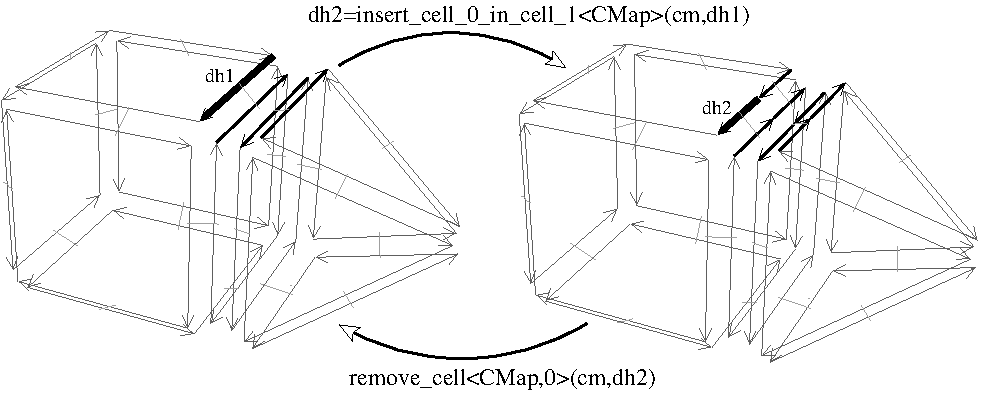
\includegraphics[width=\LargFig]{Combinatorial_map_ref/fig/pdf/insert-vertex}
%     \end{center}
%   \end{ccTexOnly}
%   \begin{ccHtmlOnly}
%     <CENTER>
%     <A HREF="fig/png/insert-vertex.png">
%         <img src="../Combinatorial_map_ref/fig/png/insert-vertex.png" alt=""></A>
%     </CENTER>
%     \end{ccHtmlOnly}
%     \centerline{Example of \ccc{insert_cell_0_in_cell_1} and \ccc{remove_cell<0>} functions.}
% %    \label{fig-exemple-remove_vertex}
% %\end{figure}

% \def\LargFig{.8\textwidth}
% %\begin{figure}
%   \begin{ccTexOnly}
%     \begin{center}
%       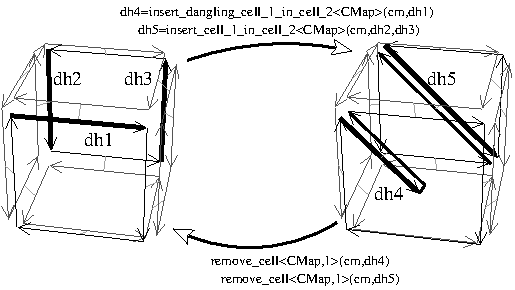
\includegraphics[width=\LargFig]{Combinatorial_map_ref/fig/pdf/insert-edge}
%     \end{center}
%   \end{ccTexOnly}
%   \begin{ccHtmlOnly}
%     <CENTER>
%     <A HREF="fig/png/insert-edge.png">
%         <img src="../Combinatorial_map_ref/fig/png/insert-edge.png" alt=""></A>
%     </CENTER>
%     \end{ccHtmlOnly}
%     \centerline{Example of \ccc{:insert_cell_1_in_cell_2} and
%       \ccc{remove_cell<1>} functions.}
% %    \label{fig-exemple-remove_edge}
% %\end{figure}

% \def\LargFig{.8\textwidth}
% %\begin{figure}
%   \begin{ccTexOnly}
%     \begin{center}
%       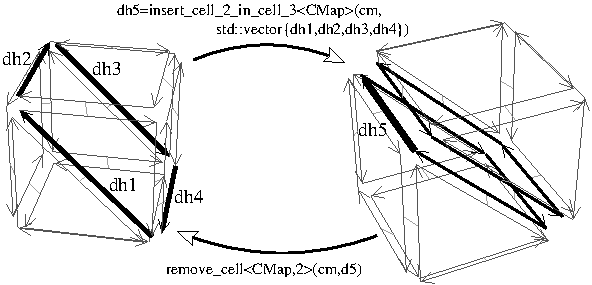
\includegraphics[width=\LargFig]{Combinatorial_map_ref/fig/pdf/insert-facet}
%     \end{center}
%   \end{ccTexOnly}
%   \begin{ccHtmlOnly}
%     <CENTER>
%     <A HREF="fig/png/insert-facet.png">
%         <img src="../Combinatorial_map_ref/fig/png/insert-facet.png" alt=""></A>
%     </CENTER>
%     \end{ccHtmlOnly}
%     \centerline{Example of \ccc{insert_cell_2_in_cell_3} and
%       \ccc{remove_cell<2>} functions.}
% %    \label{fig-exemple-remove_facet}
% %\end{figure}

\ccSeeAlso
\ccRefIdfierPage{CGAL::is_removable<CMap,i>}\\
\ccRefIdfierPage{CGAL::insert_cell_0_in_cell_1<CMap>}\\
\ccRefIdfierPage{CGAL::insert_cell_0_in_cell_2<CMap>}\\
\ccRefIdfierPage{CGAL::insert_cell_1_in_cell_2<CMap>}\\
\ccRefIdfierPage{CGAL::insert_dangling_cell_1_in_cell_2<CMap>}\\
\ccRefIdfierPage{CGAL::insert_cell_2_in_cell_3<CMap,InputIterator>}\\
\end{ccRefFunction}
%--------------------------------------------------------------------------------
\begin{ccRefFunction}{is_insertable_cell_1_in_cell_2<CMap>}
\ccInclude{CGAL/Combinatorial_map_operations.h}\\

\ccFunction{template < class CMap >
  bool is_insertable_cell_1_in_cell_2(const CMap & cm,
                       typename CMap::Dart_const_handle dh1,
                       typename CMap::Dart_const_handle dh2);}
{Returns true iff it is possible to insert a 1-cell in \ccc{cm}
  between \ccc{dh1} and \ccc{dh2}, 
  i.e. if \ccc{dh1}\myneq{}\ccc{dh2} and \ccc{dh1}\myin{}\orbit{\betaun{}}(\ccc{dh2}).
 \ccPrecond{\ccc{CMap::dimension}\mygeq{}2, 
   \ccc{*dh1}\myin{}\ccc{cm.darts()}, and \ccc{*dh2}\myin{}\ccc{cm.darts()}.}
}
% \ccCommentHeading{Template parameter}\\
% \ccc{Map} must be a model of the \ccc{CombinatorialMap} concept.
% \ccCommentHeading{Parameters} \\
% \ccc{cm}: the combinatorial map used;\\
% \ccc{dh1, dh2}: the two given darts.
% \ccCommentHeading{Returns} \\
%    true iff it is possible to insert an edge between dh1 and dh2.

\ccSeeAlso
\ccRefIdfierPage{CGAL::insert_cell_1_in_cell_2<CMap>}\\
\ccRefIdfierPage{CGAL::is_insertable_cell_2_in_cell_3<CMap,InputIterator>}\\
\end{ccRefFunction}
%--------------------------------------------------------------------------------
\begin{ccRefFunction}{is_insertable_cell_2_in_cell_3<CMap,InputIterator>}
\ccInclude{CGAL/Combinatorial_map_operations.h}\\

\ccFunction{template <class CMap, class InputIterator>
  bool is_insertable_cell_2_in_cell_3(const CMap & cm, 
     InputIterator afirst, InputIterator alast);}
{Returns true iff it is possible to insert a 2-cell in \ccc{cm} along the path
  of darts given by the range \ccc{[afirst,alast)}. The 2-cell can be inserted 
  iff each couple of consecutive darts of the path \emph{a1} and \emph{a2} belong to the 
  same vertex and the same volume, and if the path is closed.
  \ccPrecond{\ccc{CMap::dimension}\mygeq{}3.}
  % \ccCommentHeading{Template parameter}\\
  % \ccc{Map} must be a model of the \ccc{CombinatorialMap} concept.
  % \ccCommentHeading{Parameters} \\
  % \ccc{cm}: the combinatorial map used;\\
  % \ccc{afirst}: an iterator on the beginining of the path of darts.
  % \ccc{alast}: an iterator to the end of the path of darts.
  % \ccCommentHeading{Returns} \\
  % true iff it is possible to insert a facet along apath.  }
}

\ccSeeAlso
\ccRefIdfierPage{CGAL::insert_cell_2_in_cell_3<CMap,InputIterator>}\\
\ccRefIdfierPage{CGAL::is_insertable_cell_1_in_cell_2<CMap>}\\
\end{ccRefFunction}
%--------------------------------------------------------------------------------
\begin{ccRefFunction}{insert_cell_0_in_cell_1<CMap>}
\ccInclude{CGAL/Combinatorial_map_operations.h}\\

\ccFunction{template < class CMap >
  typename CMap::Dart_handle insert_cell_0_in_cell_1(CMap& cm,
                                        typename CMap::Dart_handle dh);}
{Inserts a 0-cell in the 1-cell containing \ccc{dh}. 
  Returns a handle on one dart belonging to the new 0-cell.  
  \ccPrecond{\ccc{CMap::dimension}\mygeq{}1 and \ccc{*dh}\myin{}\ccc{cm.darts()}.}\\
  See example in Figure~\ref{fig-insert-vertex}.\\
%  \begin{ccAdvanced}
    If 1-attributes are non void, 
    \ccc{Attribute_type<1>::type::On_split}(\emph{a},\emph{a'}) is called, with \emph{a} the original 1-attribute associated
    with \emph{dh} and \emph{a'} the new 1-attribute created during the operation.
%  \end{ccAdvanced}
}
%   \ccCommentHeading{Template parameter}\\
% \ccc{CMap} must be a model of the \ccc{CombinatorialMap} concept.
% \ccCommentHeading{Parameters} \\
% \ccc{cm}: the combinatorial map used;\\
% \ccc{dh}: a dart belonging to the edge.
% \ccPrecond{\ccc{can_insert_vertex<Map>(cm,dh)}}
% \ccCommentHeading{Returns} \\
%    a dart of the new vertex.
% }

\ccSeeAlso
\ccRefIdfierPage{CGAL::insert_cell_0_in_cell_2<CMap>}\\
\ccRefIdfierPage{CGAL::insert_cell_1_in_cell_2<CMap>}\\
\ccRefIdfierPage{CGAL::insert_dangling_cell_1_in_cell_2<CMap>}\\
\ccRefIdfierPage{CGAL::insert_cell_2_in_cell_3<CMap,InputIterator>}\\
\ccRefIdfierPage{CGAL::remove_cell<CMap,i>}\\
\end{ccRefFunction}
%--------------------------------------------------------------------------------
\begin{ccRefFunction}{insert_cell_0_in_cell_2<CMap>}
\ccInclude{CGAL/Combinatorial_map_operations.h}\\

\ccFunction{template <class CMap>
      typename CMap::Dart_handle insert_cell_0_in_cell_2(CMap & cm,
      typename CMap::Dart_handle dh);}
{Inserts a 0-cell in the 2-cell containing \ccc{dh}.
  The 2-cell is split in triangles, one for each initial edge of the facet.
  Returns a handle on one dart belonging to the new 0-cell.
 \ccPrecond{\ccc{CMap::dimension}\mygeq{}2 and \ccc{*dh}\myin{}\ccc{cm.darts()}.}\\
  See example in Figure~\ref{fig-triangulate}.\\
%  \begin{ccAdvanced}
    If 2-attributes are non void, 
    \ccc{Attribute_type<2>::type::On_split}(\emph{a},\emph{a'}) is called, with \emph{a} the original 2-attribute associated
    with \ccc{dh} and \emph{a'} each new 2-attribute created during the operation.
%  \end{ccAdvanced}
% \ccCommentHeading{Template parameter}\\
% \ccc{CMap} must be a model of the \ccc{CombinatorialMap} concept.
% Operation defined here is purely combinatorial, there is no geometry modification.
% \ccCommentHeading{Parameters} \\
% \ccc{cm}: the combinatorial map used;\\
% \ccc{dh}: a dart belonging to the facet to triangulate. 
% \ccCommentHeading{Returns} \\
%    a dart created during the triangulation, and incident to the new vertex.
}

\ccSeeAlso
\ccRefIdfierPage{CGAL::insert_cell_0_in_cell_2<CMap>}\\
\ccRefIdfierPage{CGAL::insert_cell_1_in_cell_2<CMap>}\\
\ccRefIdfierPage{CGAL::insert_dangling_cell_1_in_cell_2<CMap>}\\
\ccRefIdfierPage{CGAL::insert_cell_2_in_cell_3<CMap,InputIterator>}\\
\ccRefIdfierPage{CGAL::remove_cell<CMap,i>}\\
\end{ccRefFunction}
%--------------------------------------------------------------------------------
\begin{ccRefFunction}{insert_cell_1_in_cell_2<CMap>}
\ccInclude{CGAL/Combinatorial_map_operations.h}\\

\ccFunction{template < class CMap >
  typename CMap::Dart_handle insert_cell_1_in_cell_2(CMap& cm,
  typename CMap::Dart_handle dh1,typename CMap::Dart_handle dh2);}
{Inserts a 1-cell in the 2-cell containing \ccc{dh1} and \ccc{dh2}. 
  Returns \betazero{}(\ccc{dh1}), a handle on one dart belonging to the new 1-cell.  
  \ccPrecond{\ccc{is_insertable_cell_1_in_cell_2<Map>(cm,dh1,dh2)}.}\\
  See example in Figure~\ref{fig-insert-edge}.\\
%  \begin{ccAdvanced}
    If 2-attributes are non void, 
    \ccc{Attribute_type<2>::type::On_split}(\emph{a},\emph{a'}) is called, with \emph{a} the original 2-attribute associated
    with \ccc{dh} and \emph{a'} the new 2-attribute created during the operation.
%  \end{ccAdvanced}
}
%   \ccCommentHeading{Template parameter}\\
% \ccc{CMap} must be a model of the \ccc{CombinatorialMap} concept.
% \ccCommentHeading{Parameters} \\
% \ccc{cm}: the combinatorial map used;\\
% \ccc{dh1}: a first dart belonging to the facet.
% \ccc{dh2}: a second dart belonging to the facet.
% \ccPrecond{\ccc{can_insert_edge<Map>(cm,dh1,dh2)}}
% \ccCommentHeading{Returns} \\
%    a dart of the new edge.}

\ccSeeAlso
\ccRefIdfierPage{CGAL::is_insertable_cell_1_in_cell_2<CMap>}\\
\ccRefIdfierPage{CGAL::insert_cell_0_in_cell_1<CMap>}\\
\ccRefIdfierPage{CGAL::insert_cell_0_in_cell_2<CMap>}\\
\ccRefIdfierPage{CGAL::insert_dangling_cell_1_in_cell_2<CMap>}\\
\ccRefIdfierPage{CGAL::insert_cell_2_in_cell_3<CMap,InputIterator>}\\
\ccRefIdfierPage{CGAL::remove_cell<CMap,i>}\\
\end{ccRefFunction}
%--------------------------------------------------------------------------------
\begin{ccRefFunction}{insert_dangling_cell_1_in_cell_2<CMap>}
\ccInclude{CGAL/Combinatorial_map_operations.h}\\

\ccFunction{template < class CMap >
  typename CMap::Dart_handle insert_dangling_cell_1_in_cell_2(CMap& cm,
                                         typename CMap::Dart_handle dh);}
{Inserts a 1-cell in a the 2-cell containing \ccc{dh}, the 1-cell
being attached only by one of its extremity to the 0-cell containing \ccc{dh}.
  Returns a handle on one dart belonging to the new 1-cell.
 \ccPrecond{\ccc{CMap::dimension}\mygeq{}2 and \ccc{*dh}\myin{}\ccc{cm.darts()}.}\\
  See example in Figure~\ref{fig-insert-edge}.
}
%   \ccCommentHeading{Template parameter}\\
% \ccc{CMap} must be a model of the \ccc{CombinatorialMap} concept.
% \ccCommentHeading{Parameters} \\
% \ccc{cm}: the combinatorial map used;\\
% \ccc{dh}: a dart belonging to the facet.
% \ccCommentHeading{Returns} \\
%    a dart of the new edge and incident to the new vertex.}

\ccSeeAlso
\ccRefIdfierPage{CGAL::insert_cell_0_in_cell_1<CMap>}\\
\ccRefIdfierPage{CGAL::insert_cell_0_in_cell_2<CMap>}\\
\ccRefIdfierPage{CGAL::insert_cell_1_in_cell_2<CMap>}\\
\ccRefIdfierPage{CGAL::insert_cell_2_in_cell_3<CMap,InputIterator>}\\
\ccRefIdfierPage{CGAL::remove_cell<CMap,i>}\\
\end{ccRefFunction}
%--------------------------------------------------------------------------------
\begin{ccRefFunction}{insert_cell_2_in_cell_3<CMap,InputIterator>}
\ccInclude{CGAL/Combinatorial_map_operations.h}\\

\ccFunction{template <class CMap, class InputIterator>
  typename CMap::Dart_handle insert_cell_2_in_cell_3(CMap & cm,
                            InputIterator afirst, InputIterator alast);}
{Inserts a 2-cell along the path of 1-cells containing darts given 
  by the range \ccc{[afirst,alast)}.
  Returns a handle on one dart belonging to the new 2-cell.  
  \ccPrecond{\ccc{is_insertable_cell_2_in_cell_3<Map>(cm,afirst,alast)}.}\\
  See example in Figure~\ref{fig-insert-face}.\\
%  \begin{ccAdvanced}
    If 3-attributes are non void, 
    \ccc{Attribute_type<3>::type::On_split}(\emph{a},\emph{a'}) is called, with \emph{a} the original 3-attribute associated
    with \ccc{dh} and \emph{a'} the new 3-attribute created during the operation.
%  \end{ccAdvanced}
}
% \ccCommentHeading{Template parameter}\\
% \ccc{CMap} must be a model of the \ccc{CombinatorialMap} concept.
% \ccCommentHeading{Parameters} \\
% \ccc{cm}: the combinatorial map used;\\
% \ccc{afirst}: an iterator on the beginining of the path of darts.
% \ccc{alast}: an iterator to the end of the path of darts.
% \ccPrecond{\ccc{can_insert_facet<Map>(cm,afirst,alast)}}
% \ccCommentHeading{Returns} \\
%     a dart of the new facet.}

\ccSeeAlso
\ccRefIdfierPage{CGAL::is_insertable_cell_2_in_cell_3<CMap,InputIterator>}\\
\ccRefIdfierPage{CGAL::insert_cell_0_in_cell_1<CMap>}\\
\ccRefIdfierPage{CGAL::insert_cell_0_in_cell_2<CMap>}\\
\ccRefIdfierPage{CGAL::insert_cell_1_in_cell_2<CMap>}\\
\ccRefIdfierPage{CGAL::insert_dangling_cell_1_in_cell_2<CMap>}\\
\ccRefIdfierPage{CGAL::remove_cell<CMap,i>}\\
\end{ccRefFunction}
%--------------------------------------------------------------------------------

% +------------------------------------------------------------------------+
%%RefPage: end of main body, begin of footer
\ccRefPageEnd
% EOF
% +------------------------------------------------------------------------+
